\documentclass{beamer}


%%% EU logo
% small version for upper right corner of normal pages
\pgfdeclareimage[width=12.8cm]{university-logo}{JRC_header}
\logo{\pgfuseimage{university-logo}}
\pgfdeclareimage[height=5.5mm]{footimage}{JRC_footer}
\newcommand{\titleimage}[1]{\pgfdeclareimage[width=0.5\textwidth]{title-image}{#1}}
%\newcommand{\footimage}{\pgfdeclareimage[width=0.5\textwidth]{title-image}{#1}}
\titlegraphic{\pgfuseimage{title-image}}
%%% end EU logo

% NOTE: 1cm = 0.393 in = 28.346 pt;    1 pt = 1/72 in = 0.0352 cm
\setbeamersize{text margin right=3.5mm, text margin left=7.5mm}  % text margin

% colors to be used
\definecolor{text-grey}{rgb}{0.45, 0.45, 0.45} % grey text on white background
\definecolor{bg-grey}{rgb}{0.66, 0.65, 0.60} % grey background (for white text)
\definecolor{eu-blue}{RGB}{55, 172, 222} % blue text
\definecolor{drk-blue}{RGB}{0, 51, 102} % blue text
\definecolor{fu-blue}{RGB}{0, 51, 102} % blue text
\definecolor{fu-green}{RGB}{153, 204, 0} % green text
\definecolor{fu-red}{RGB}{204, 0, 0} % red text (used by \alert)

% switch off the sidebars
\setbeamersize{sidebar width left=0cm, sidebar width right=0mm}
\setbeamertemplate{sidebar right}{}
\setbeamertemplate{sidebar left}{}
\setbeamertemplate{navigation symbols}{}%remove navigation symbols

% frame title
\setbeamertemplate{frametitle}{%
    \vskip-5pt \color{drk-blue}\Large%
    \begin{minipage}[b][23pt]{\textwidth}%
    \flushleft \textbf{\insertframetitle}%
    \end{minipage}%
}

%%% title page
\setbeamertemplate{title page}{

% set the title
\parbox[top][2.8cm][c]{\textwidth}{\begin{center} \color{drk-blue}\LARGE \textbf{\inserttitle}  \\ \vspace{10pt} \small \insertsubtitle \end{center}}

% title image of the presentation
\begin{minipage}{0.5\textwidth}
\flushleft
%\hspace{-7.5mm}
\inserttitlegraphic
\end{minipage}
% Author info
\hspace{0.5cm}
\begin{minipage}{0.4\textwidth}
{\flushleft \color{black} \textbf{\insertauthor} \\ \insertinstitute }
\end{minipage}
}
%%% end title page

%%% colors
\usecolortheme{lily}
\setbeamercolor*{normal text}{fg=drk-blue, bg=white}
\setbeamercolor*{alerted text}{fg=fu-red}
\setbeamercolor*{example text}{fg=fu-green}
\setbeamercolor*{structure}{fg=fu-blue}

\setbeamercolor*{block title}{fg=white,bg=black!50}
\setbeamercolor*{block title alerted}{fg=white,bg=black!50}
\setbeamercolor*{block title example}{fg=white,bg=black!50}

\setbeamercolor*{block body}{bg=black!10}
\setbeamercolor*{block body alerted}{bg=black!10}
\setbeamercolor*{block body example}{bg=black!10}

\setbeamercolor{item}{fg=eu-blue}
%%% end colors

\setbeamertemplate{itemize items}[circle] % if you want a ball
\setbeamertemplate{itemize subitem}[circle] % if you wnat a circle
\setbeamertemplate{itemize subsubitem}[cirlce] % if you want a triangle

%%% headline
\setbeamertemplate{headline}{
\insertlogo % logo on the right
%\begin{center}
%\colorbox{eu-blue}{
% \begin{minipage}[t]{.8\textwidth} \color{eu-blue} text \vspace{25pt} %\end{minipage}}
%\begin{minipage}[c]{0.0\textwidth}
%\hspace{-10mm} hi
%\end{minipage}
%\end{center}
}
%%% end headline

%%% footline
\newcommand{\footlinetext}{\insertdate}
\setbeamertemplate{footline}{
\begin{minipage}{58mm}
 \color{drk-blue} \hspace{7.5mm} \footlinetext
\end{minipage}
\hspace{0.1mm} 
\begin{minipage}{8.5mm}
 \pgfuseimage{footimage}
\end{minipage}
\hspace{0.1mm}
\begin{minipage}{50mm}
 \color{drk-blue} 
 %\raisebox{-1pt}{\usebeamertemplate***{navigation symbols}}
 \flushright \insertframenumber
\end{minipage}

}
%%% end footline
 
\usepackage{arev,t1enc}
\usepackage{amsmath}

\usepackage[T1]{fontenc}
\fontfamily{verdana}\selectfont

\title{The Costs of Ignoring Stock Structure}
%\subtitle{}
\author{Colin Millar\\Ernesto Jardim\\Iago Mosqueira\\Chato Osio}
\institute{European Commission\\ Joint Research Center}
\subject{Fisheries Management}

\usepackage{Sweave}
\begin{document}
\setkeys{Gin}{width=1.1\textwidth}

%% set up R environment
%<<echo=FALSE, results=hide>>=
%library(RColorBrewer)
%library(lattice)
%library(xtable)
%library(Hmisc)
%load("../presentation-data.rda")
%@

%%%%%%%%%%%%%%%%%%%%%%%%%%%%%%%%%%%%%%%%%%%%%

\begin{frame}
\titlepage
\end{frame}

%%%%%%%%%%%%%%%%%%%%%%%%%%%%%%%%%%%%%%%%%%%%%

%\begin{withoutheadline}
%\begin{frame}{}
%  \begin{center}
%  \begin{minipage}{.7\textwidth}
%    \centering
%    \LARGE \textit{All myths are true, \\ for a given value of 'true'}
%    \flushright
%    \LARGE \textit{Pratchett, 1998}
%   \end{minipage}
%  \end{center}
%\end{frame}
%\end{withoutheadline}

\begin{withoutheadline}
\begin{frame}{Motivation}
  %a4a Initiative with brief description - 1st two paras of docs.  Keyword is 2020 because by then we will have time series of 10 to 15 years for most exploited European fish stocks.  Keyword management advice for moderate data stocks - this is a stock with time series of 10-15 yrs one index and info on growth and maturity. 
  \begin{itemize}
    \item The \textbf{a4a initiative} aims to provide methods to manage stocks with \textbf{moderate data} series (10 - 15 years)
    \item One of the discussions is about how \textbf{genetics} can help in \textbf{management}
    \item Currently the most powerful application of Genetic analysis in fisheries management is in \textbf{identifying sub-stocks}
  \end{itemize}
\end{frame}
\end{withoutheadline}

\begin{withoutheadline}
\begin{frame}{}
\begin{center}
\LARGE \textbf{But what are the impacts of managing (or not) sub-stocks ?}
\end{center}
\end{frame}
\end{withoutheadline}


\begin{withoutheadline}
\begin{frame}{Aims}

  Focusing on the problem of sub units having different life histories and productivities while living in reproductive isolation

  \begin{itemize}
      \item Investigate managing two sub-units as one stock
      \item or equivalently, two stocks managed as one stock
  \end{itemize}

  \pause  
  Mixed species
  \begin{itemize}
    \item \textit{Lophius piscatorius} and \textit{L. budagassa}
    \item \textit{Scomber scombrus} and \textit{Scomber japonicus}
  \end{itemize}
  \vspace{.25cm}
  Mixed sub-units
  \begin{itemize}
    \item Atlantic Blue-Fin Tuna, Mediterranean or Gulf of Mexico
    \item Atlantic Cod ?
    \item North Sea Whiting ?
  \end{itemize}

\end{frame}
\end{withoutheadline}

\begin{withoutheadline}
\begin{frame}{Secondary Aims}
  \begin{itemize}
      \item achieve some a4a initiative objectives
      \item develop a statistical catch at age model
      \item develop a (flexible) testing framework
      \item develop an MSE algorithm
  \end{itemize}
\end{frame}
\end{withoutheadline}


\begin{withoutheadline}
\begin{frame}{Outline}
  \begin{itemize}
    \item Simulation Design
    \item Simulating a range of realistic stock: choosing plausible parameter values
    \item Brief look at the scenarios
    \item Results    
    \begin{itemize}
      \item Investigate the proportion in the biomass at the end of a 30 year simulation
      \item Investigate stock status in comparison to the case of no difference in sub units
    \end{itemize}
%    \item Some final thoughts
  \end{itemize}
\end{frame}
\end{withoutheadline}


%%%%%%%%%%%%%%%%%%%%%%%%%%%%%%%%%%%%%%%%%%%%%

\begin{withoutheadline}
\begin{frame}{Simulation Design}
  The MSE diagram
  \begin{figure}
    \centering
    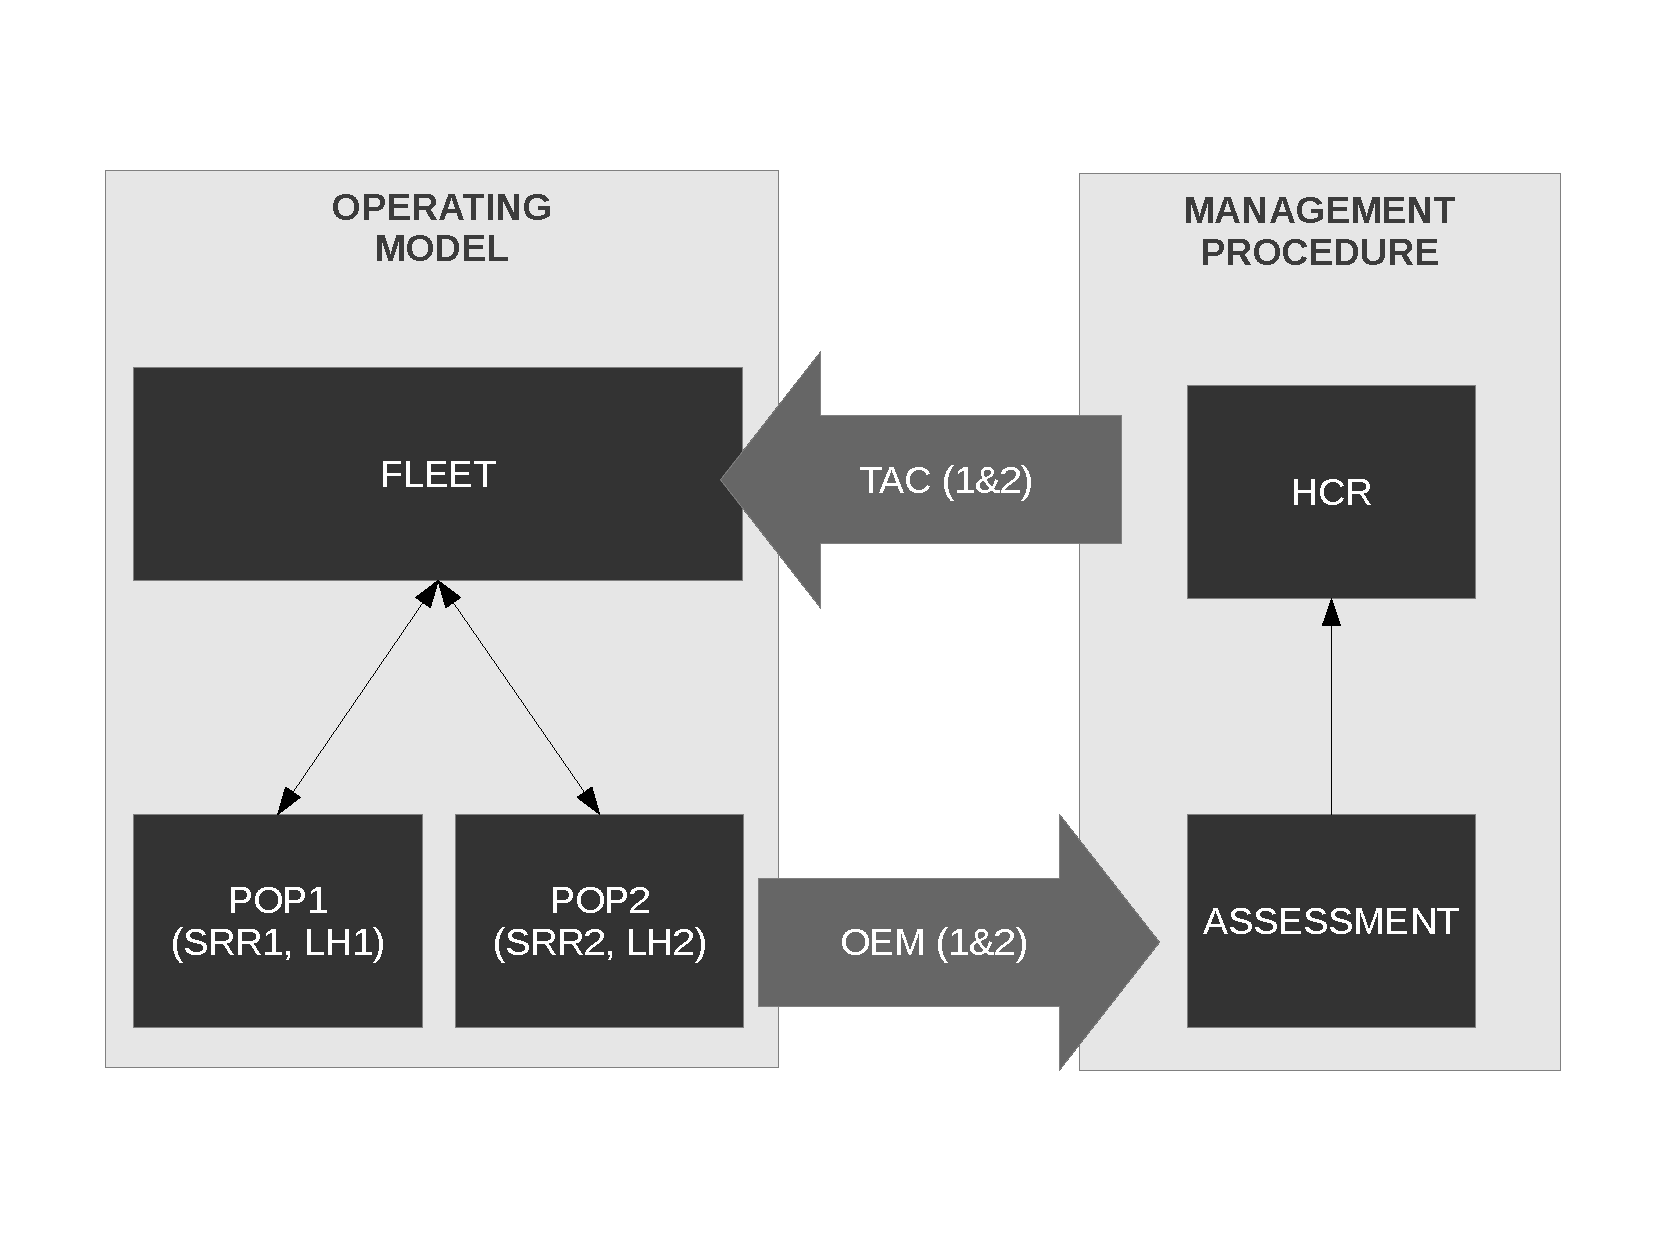
\includegraphics[width=.9\textwidth]{mse02}
  \end{figure}
\end{frame}
\end{withoutheadline}


%\begin{withoutheadline}
%\begin{frame}{Population model}
%  The Population Model for one unit
%  \begin{figure}
%    \centering
%    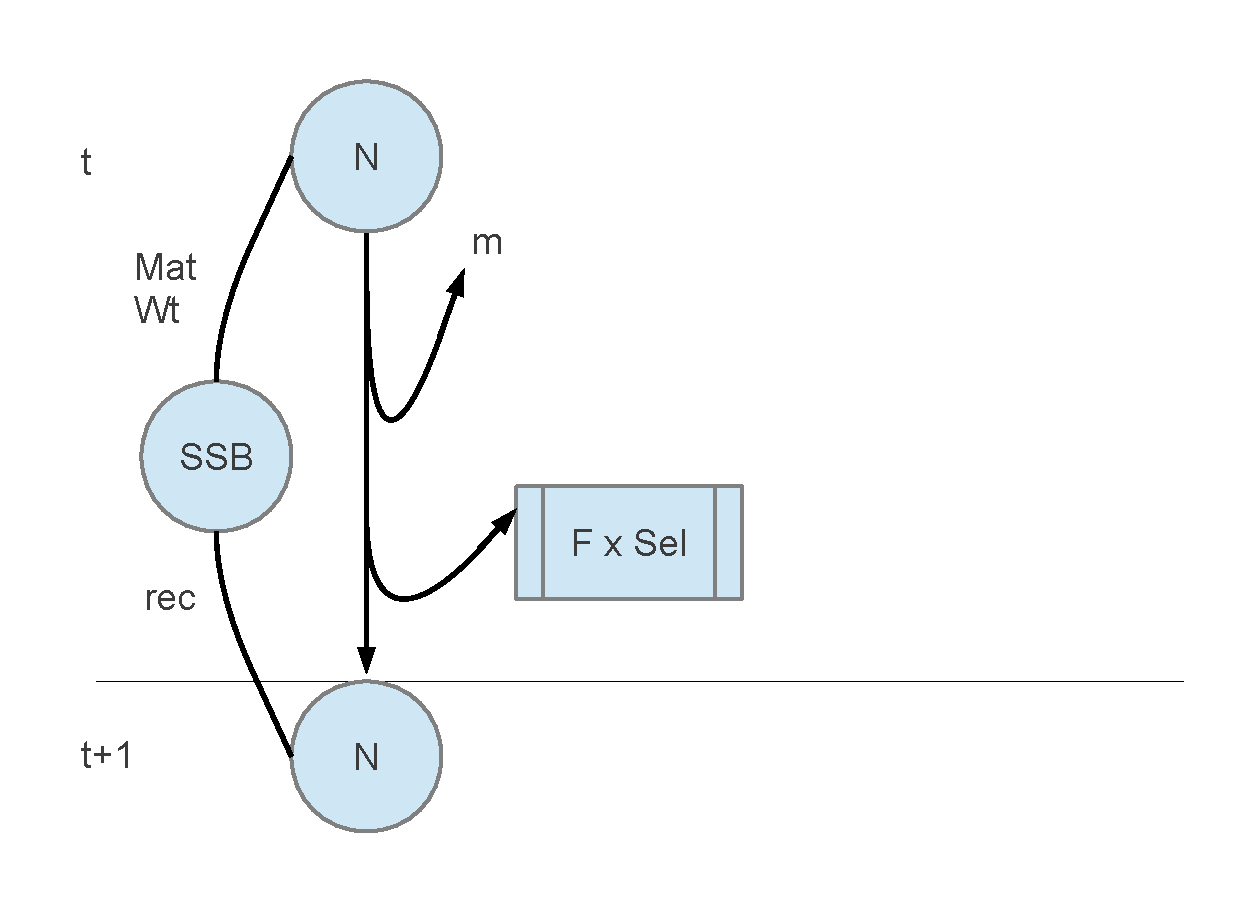
\includegraphics[width=.9\textwidth]{Population-model-half}
%  \end{figure}
%\end{frame}
%\end{withoutheadline}
%
%
%\begin{withoutheadline}
%\begin{frame}{Population model}
%  The Population Model for two units
%  \begin{figure}
%    \centering
%    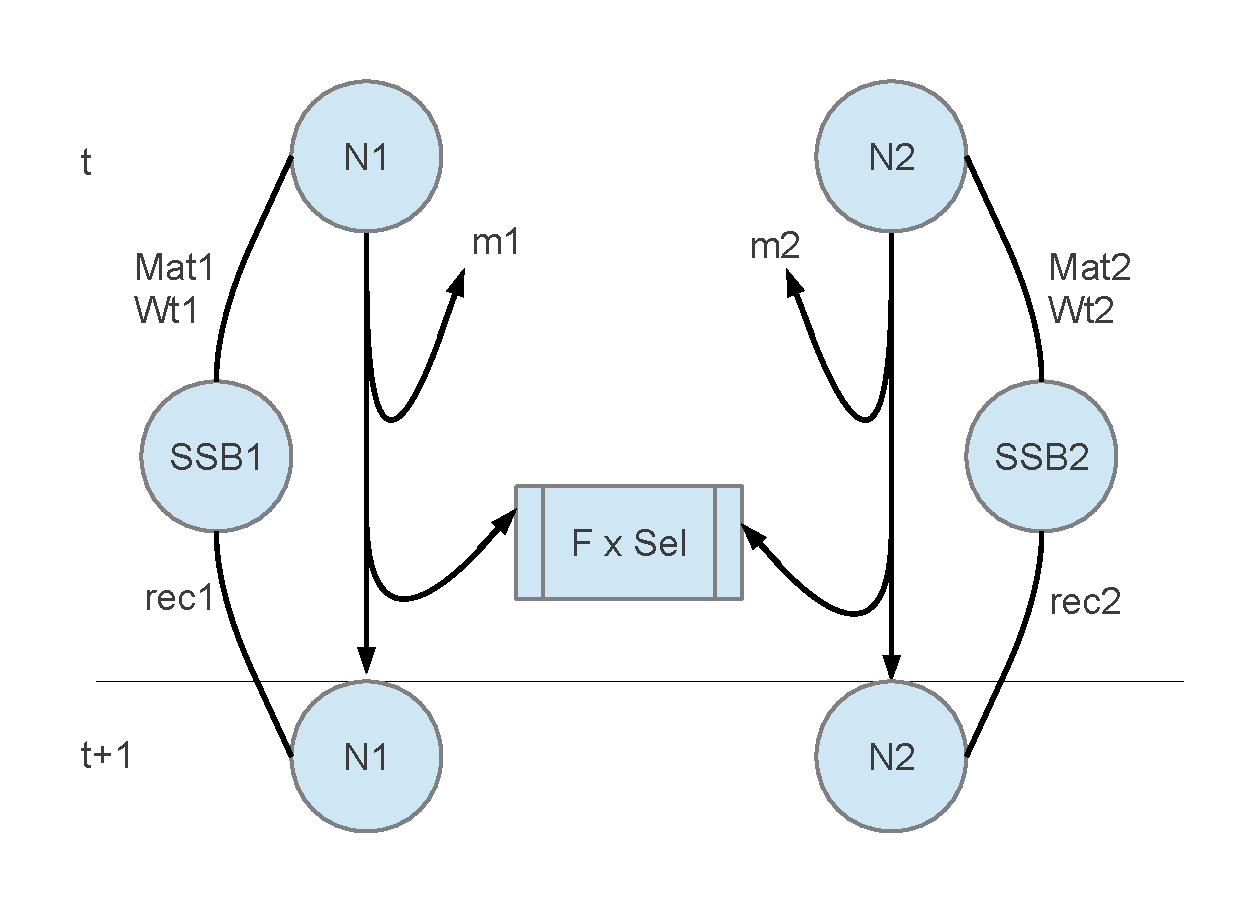
\includegraphics[width=.9\textwidth]{Population-model}
%  \end{figure}
%\end{frame}
%\end{withoutheadline}


%\begin{withoutheadline}
%\begin{frame}{Observation and Management Procedure}
%  We observe  
%  \begin{itemize}
%    \item combined catch
%    \item index of combined abundance
%    \item combined mean weight at age
%    \item average M and maturity
%  \end{itemize}
%  \vspace{.25cm}
%  TAC is based on
%  \begin{itemize}
%    \item F and SSB estimate from a statistical catch at age model
%    \item a harvest control rule with annually estimated reference points
%    \item assuming geometric mean recruitment
%    \item mean weight at age over last three years
%    \item assuming current TAC taken in intermediate year
%  \end{itemize}
%\end{frame}
%\end{withoutheadline}

%%%%%%%%%%%%%%%%%%%%%%%%%%%%%%%%%%%%%%%%%%%%%

\begin{withoutheadline}
\begin{frame}{The Harvest Control Rule}
  \begin{figure}
    \begin{center}
    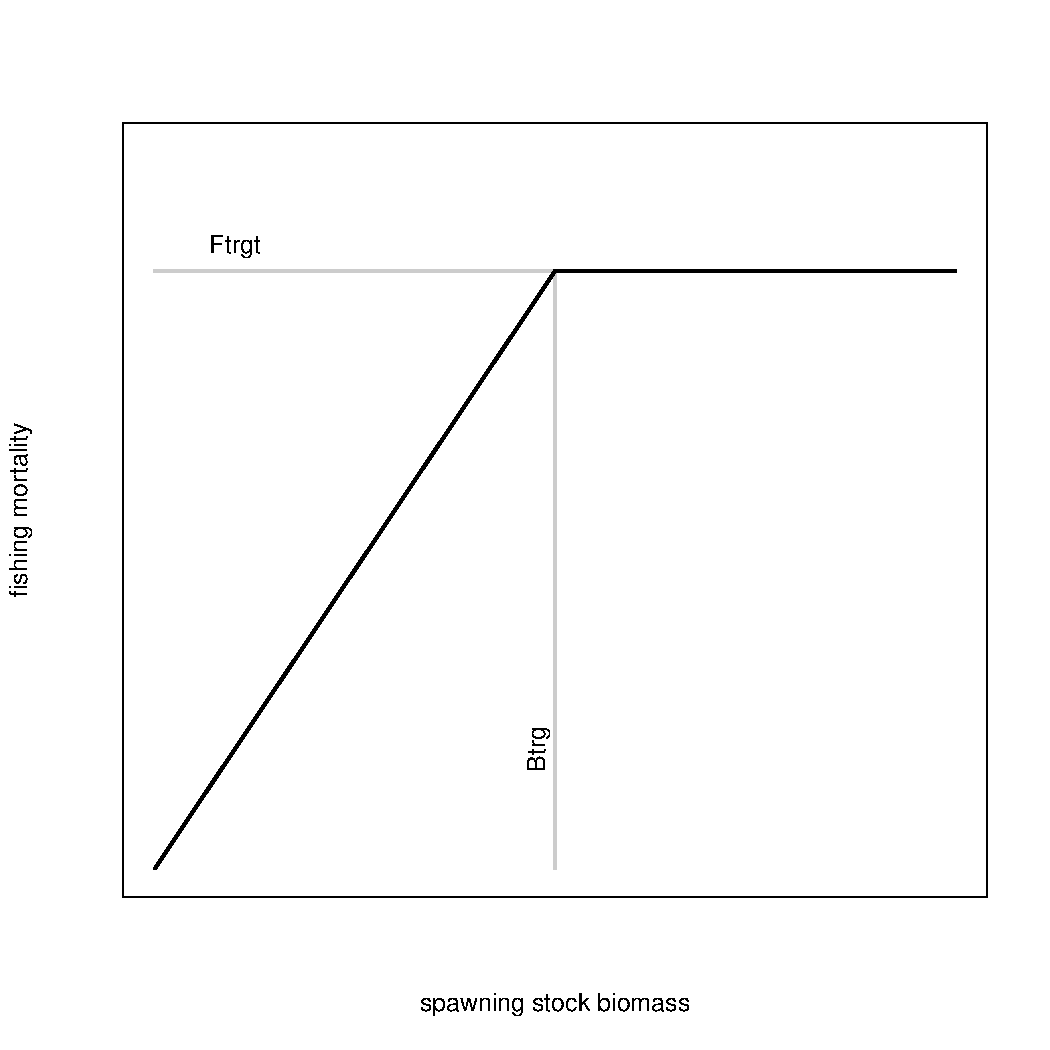
\includegraphics[width=.65\textwidth]{hcr}    
    \end{center}
  \end{figure}
\end{frame}
\end{withoutheadline}


%%%%%%%%%%%%%%%%%%%%%%%%%%%%%%%%%%%%%%%%%%%%%

\begin{withoutheadline}
\begin{frame}{Choosing Parameter Values}
  \begin{itemize}
    \item Used relationships in Gislason et al. 2008 \footnote{Gislason, H., Pope, J. G., Rice, J. C., and Daan, N. 2008. Coexistence in North Sea fish communities: implications for growth and natural mortality. ICES Journal of Marine Science, 65: 514-530.}
    \item weight length values from FishBase
    \item recruitment levels - ICES north sea estimates as guide
    \item Stock recruit curve shapes designed to be viable under fishing
  \end{itemize}
\end{frame}
\end{withoutheadline}

\begin{withoutheadline}
\begin{frame}{The Simulated Sub Stock Units}
  \begin{minipage}{.3\textwidth}
   Growth params:\\
   Linf = 60, 80, 100 cm \\
   T0 = -1 \\
   
   \vspace{.25cm}
   WLR:\\ a = $5e^{-6}$ and b = 2.9 \\

   \vspace{.25cm}   
   fishery selection:\\ trawl-like \\
   full selection at age 4  
  \end{minipage}
  \hspace{0.25cm}  
  \begin{minipage}{.65\textwidth}
  \begin{figure}
  \flushleft
  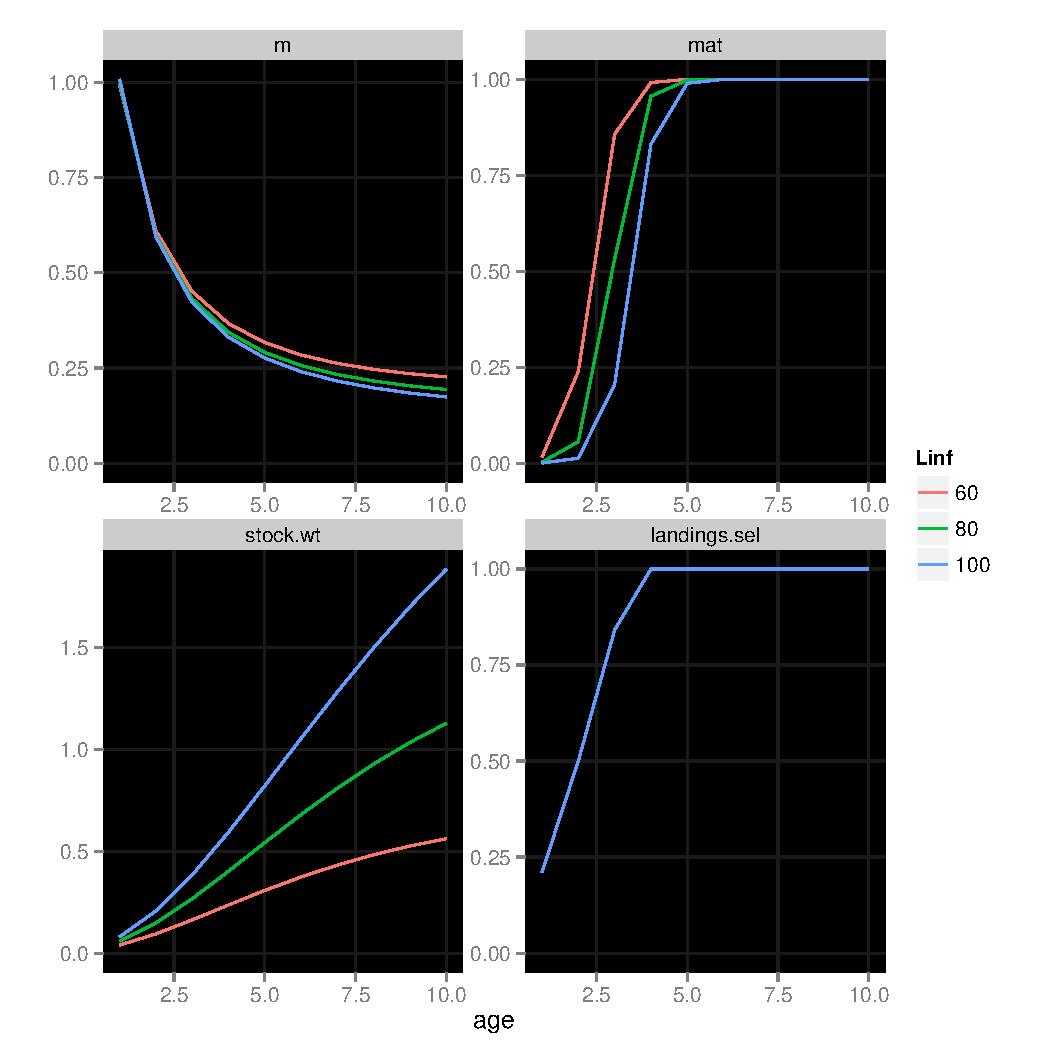
\includegraphics[width=\textwidth]{LH-choices1}
  \end{figure}
  \end{minipage}
\end{frame}
\end{withoutheadline}

\begin{withoutheadline}
\begin{frame}{The Simulated Sub Stock Units}
  \begin{minipage}{.3\textwidth}
   Max recruits: \\
   at 350 and 525 million \\

   \vspace{.25cm}   
   made slopes at low biomasses similar
   for comparability
  \end{minipage}
  \hspace{0.25cm}  
  \begin{minipage}{.65\textwidth}
  \begin{figure}
  \flushleft
  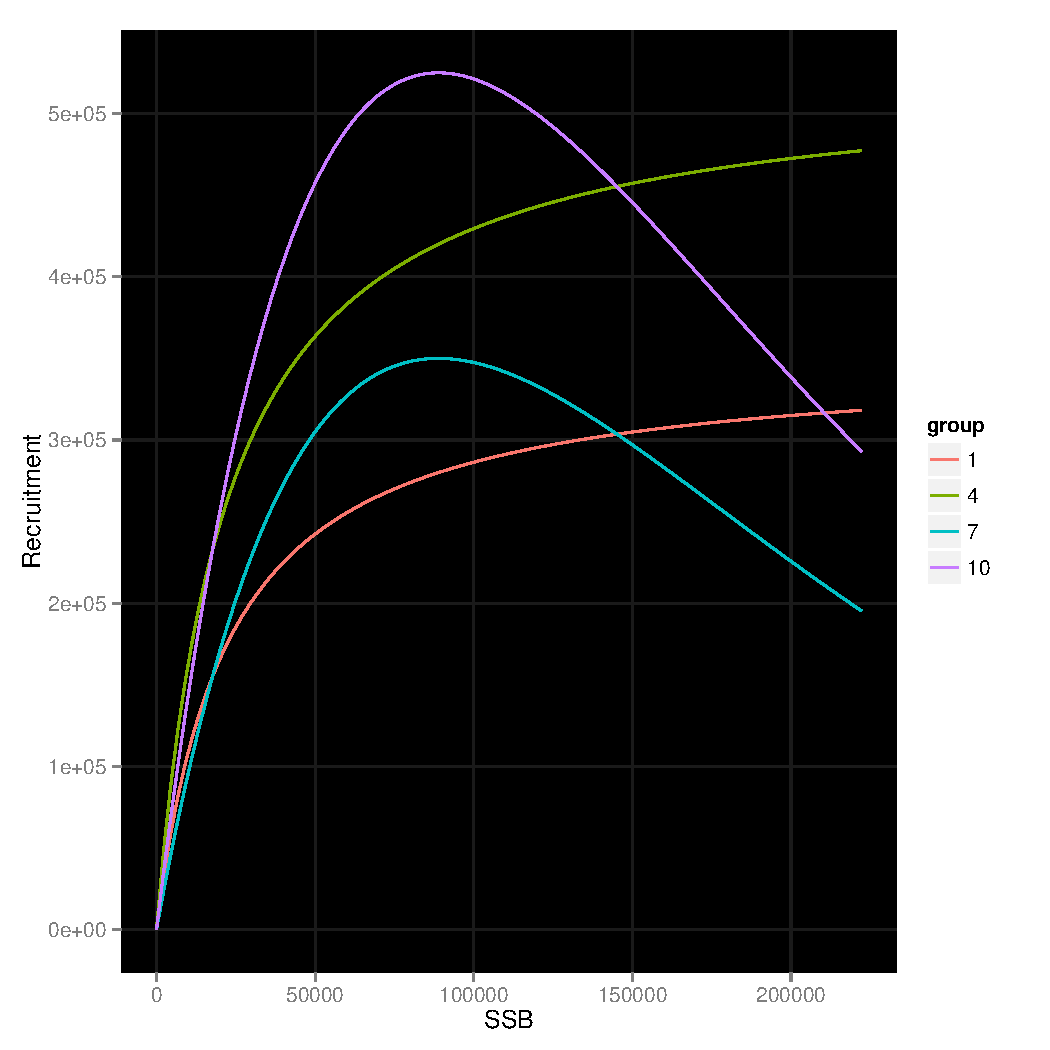
\includegraphics[width=\textwidth]{LH-choices2}
  \end{figure}
  \end{minipage}
\end{frame}
\end{withoutheadline}


%%%%%%%%%%%%%%%%%%%%%%%%%%%%%%%%%%%%%%%%%%%%%

\begin{withoutheadline}
\begin{frame}{Simulated Sub Stock Units}
  \begin{minipage}{.3\textwidth}
    The starting point for the simulations was at 40 yrs
  \end{minipage}
  \hspace{0.25cm}  
  \begin{minipage}{.65\textwidth}
  \begin{figure}
  \flushleft
  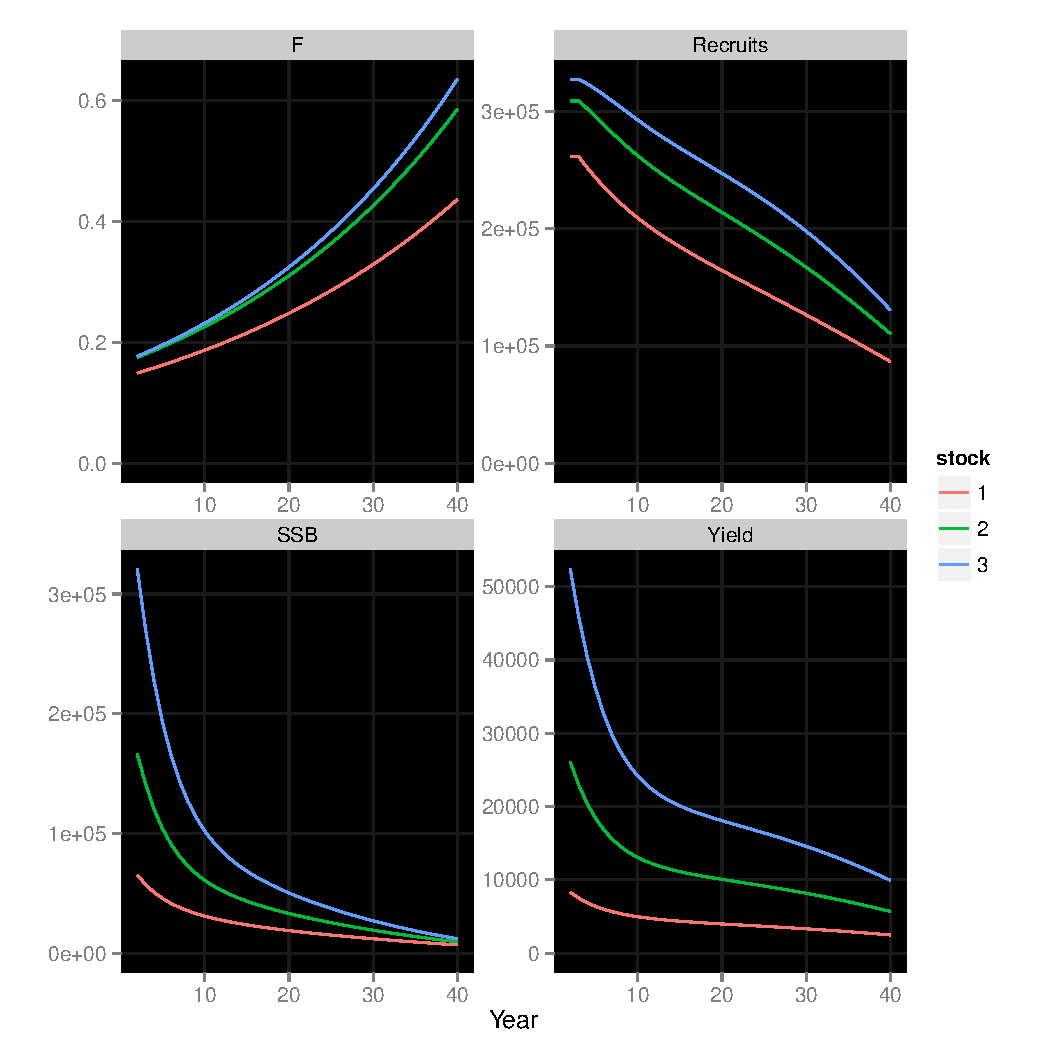
\includegraphics[width=\textwidth]{stock-unit1}
  \end{figure}
  \end{minipage}
\end{frame}
\end{withoutheadline}


%%%%%%%%%%%%%%%%%%%%%%%%%%%%%%%%%%%%%%%%%%%%%

\begin{withoutheadline}
\begin{frame}{Scenarios}
We simulated with all combinations of:\\

\vspace{.25cm}
\begin{itemize}
\item[ ] Linf: 60, 80 and 100 cm
\item[ ] Recruitment: low and high
\end{itemize}
\vspace{.25cm}
This resulted in 6 sub units giving 21 comparisons \\
\vspace{.5cm}
This was done separately for the Beverton-Holt and the Ricker models
\end{frame}
\end{withoutheadline}

\begin{withoutheadline}
\begin{frame}{Scenarios}
  \begin{figure}
  \flushright
    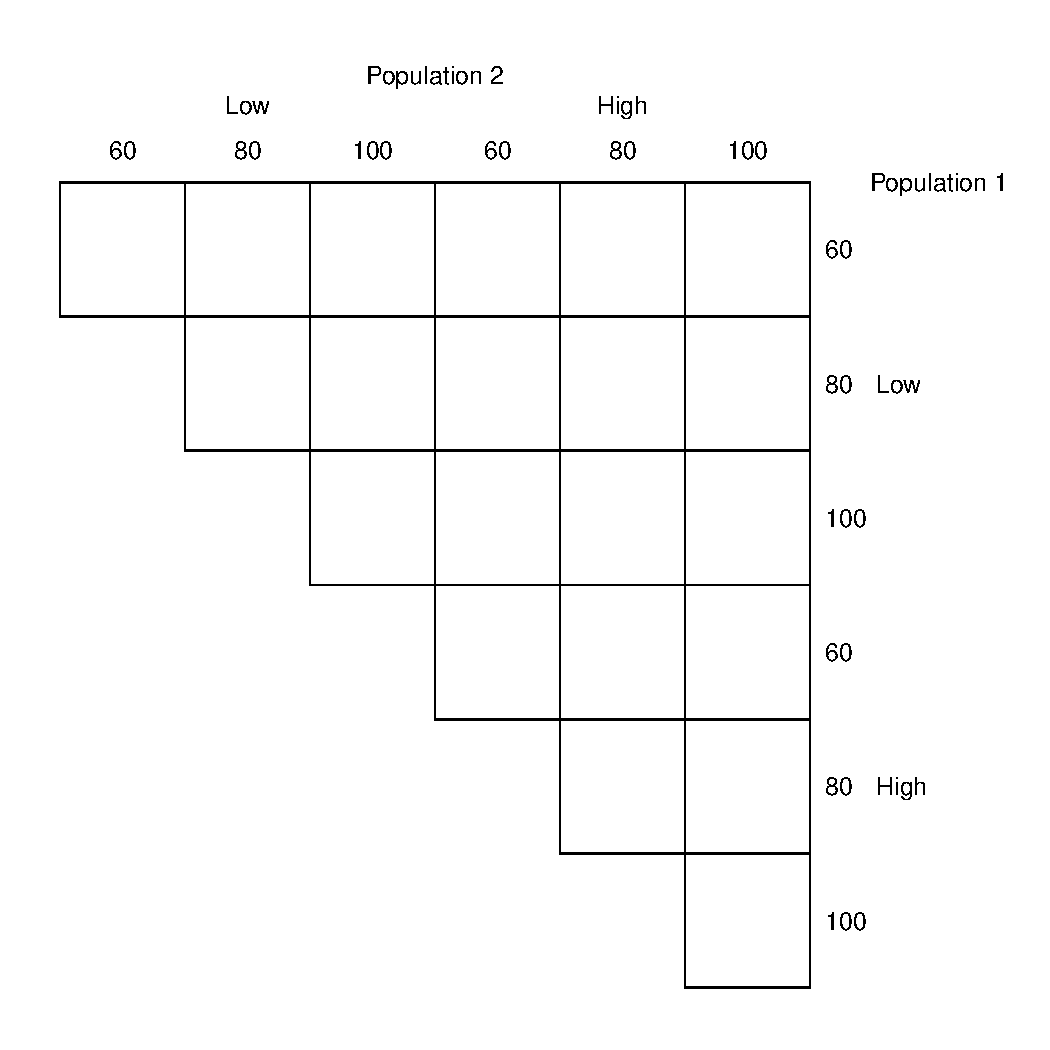
\includegraphics[width=.7\textwidth]{scenario0}
  \end{figure}
\end{frame}
\end{withoutheadline}

\begin{withoutheadline}
\begin{frame}{Scenarios: controls}
  \begin{figure}
  \flushright
    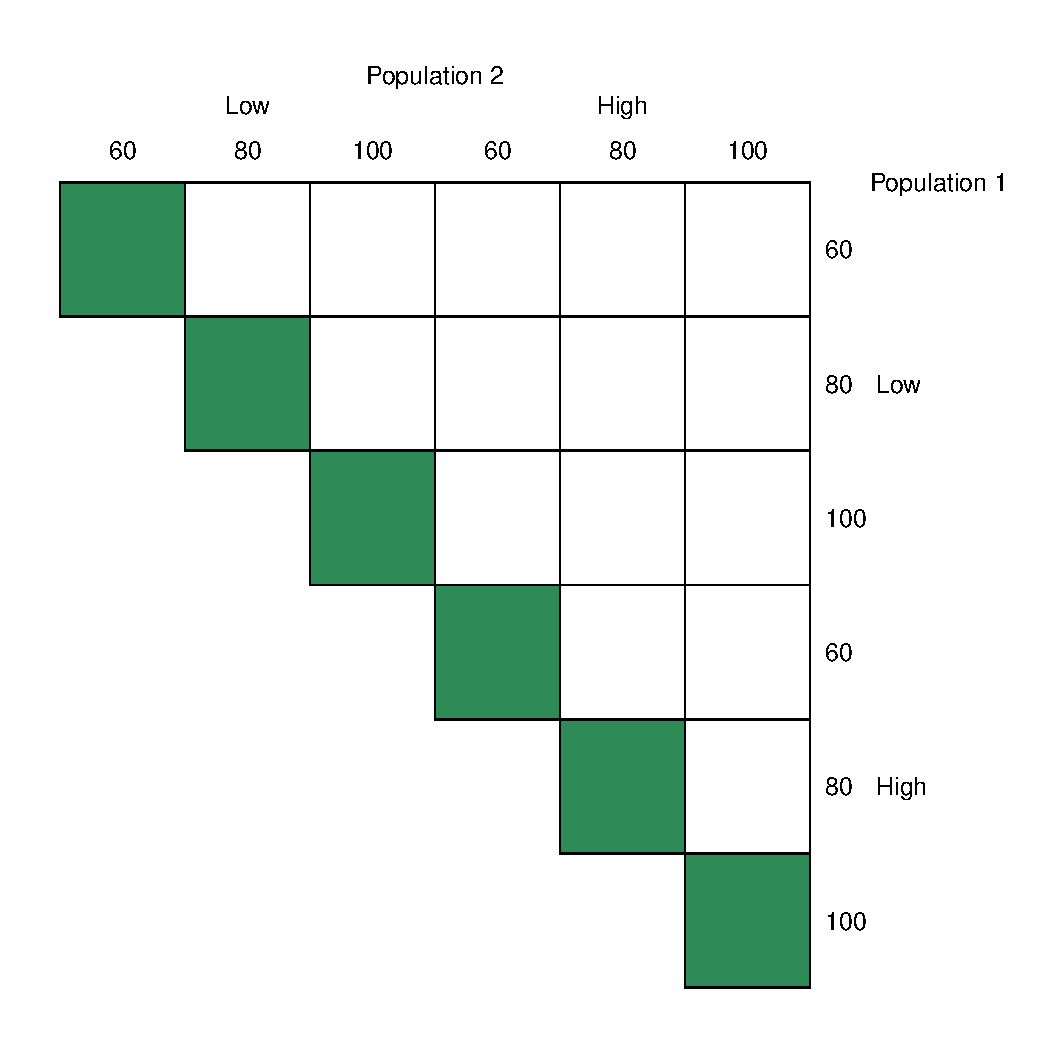
\includegraphics[width=.7\textwidth]{scenario1}
  \end{figure}
\end{frame}
\end{withoutheadline}

\begin{withoutheadline}
\begin{frame}{Scenarios: growth comparisons}
  \begin{figure}
  \flushright
    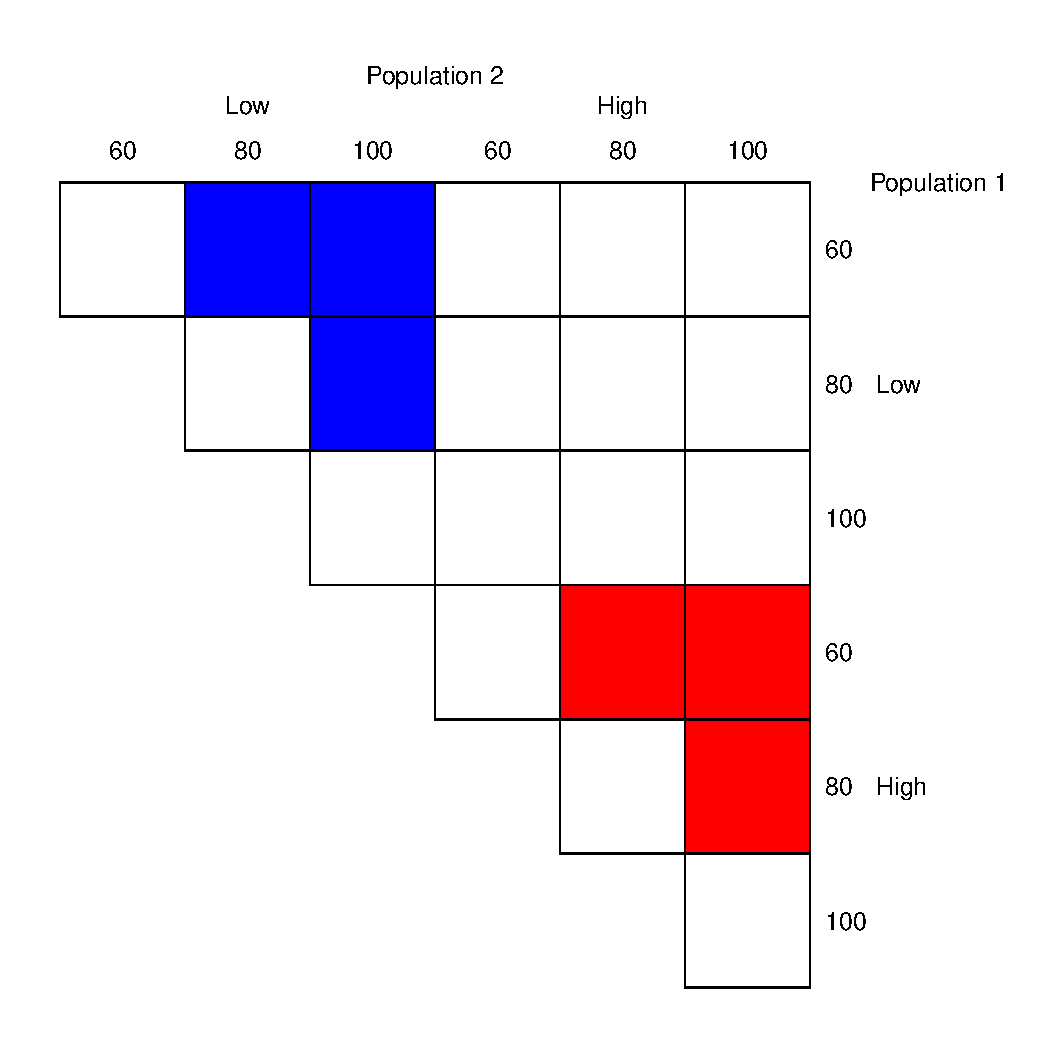
\includegraphics[width=.7\textwidth]{scenario2}
  \end{figure}
\end{frame}
\end{withoutheadline}

\begin{withoutheadline}
\begin{frame}{Scenarios: Productivity}
  \begin{figure}
  \flushright
    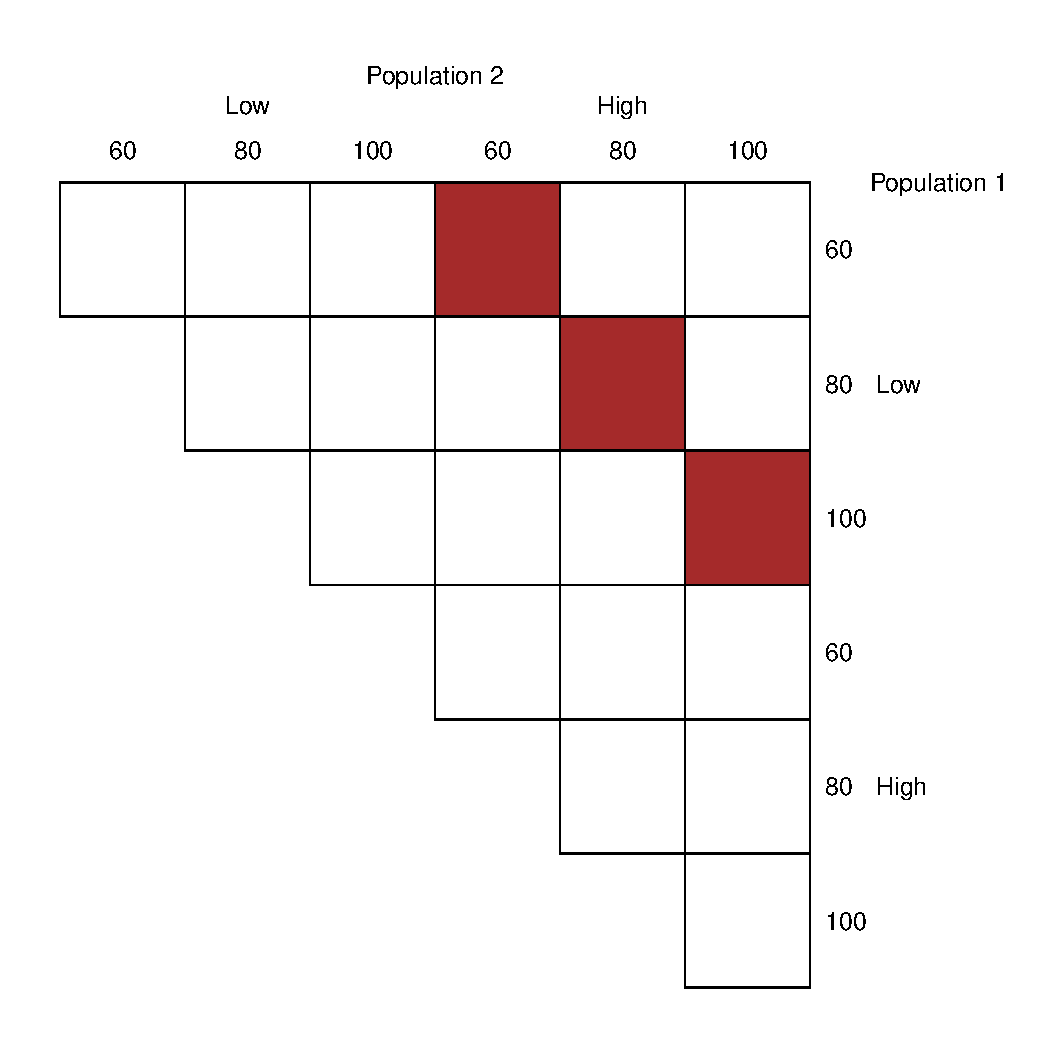
\includegraphics[width=.7\textwidth]{scenario3}
  \end{figure}
\end{frame}
\end{withoutheadline}

\begin{withoutheadline}
\begin{frame}{Scenarios: interaction of growth and productivity}
  \begin{figure}
  \flushright
    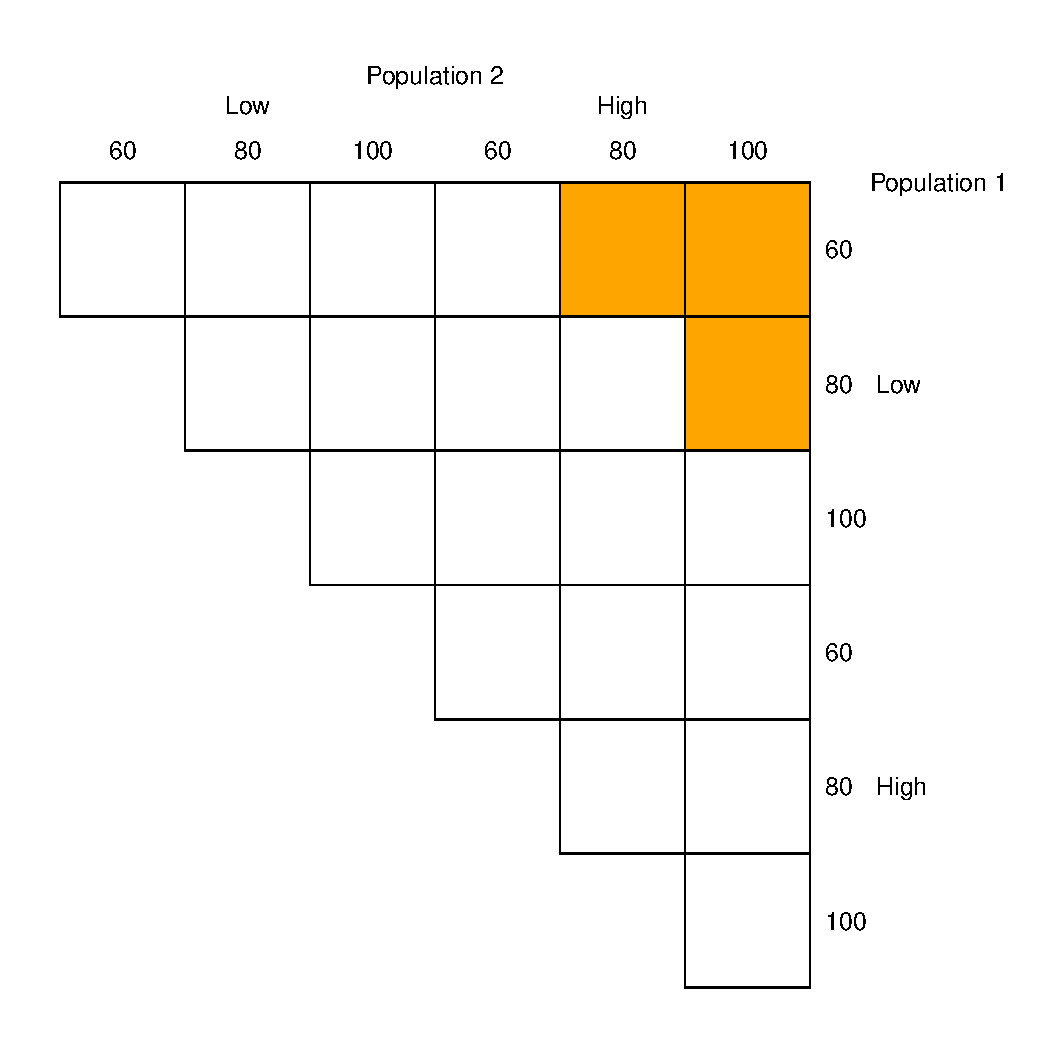
\includegraphics[width=.7\textwidth]{scenario4}
  \end{figure}
\end{frame}
\end{withoutheadline}


%%%%%%%%%%%%%%%%%%%%%%%%%%%%%%%%%%%%%%%%%%%%%

\begin{withoutheadline}
\begin{frame}{Results}
  Two sub-units with Linf = 60 and low BH recruitment
  \begin{figure}
  \flushright
  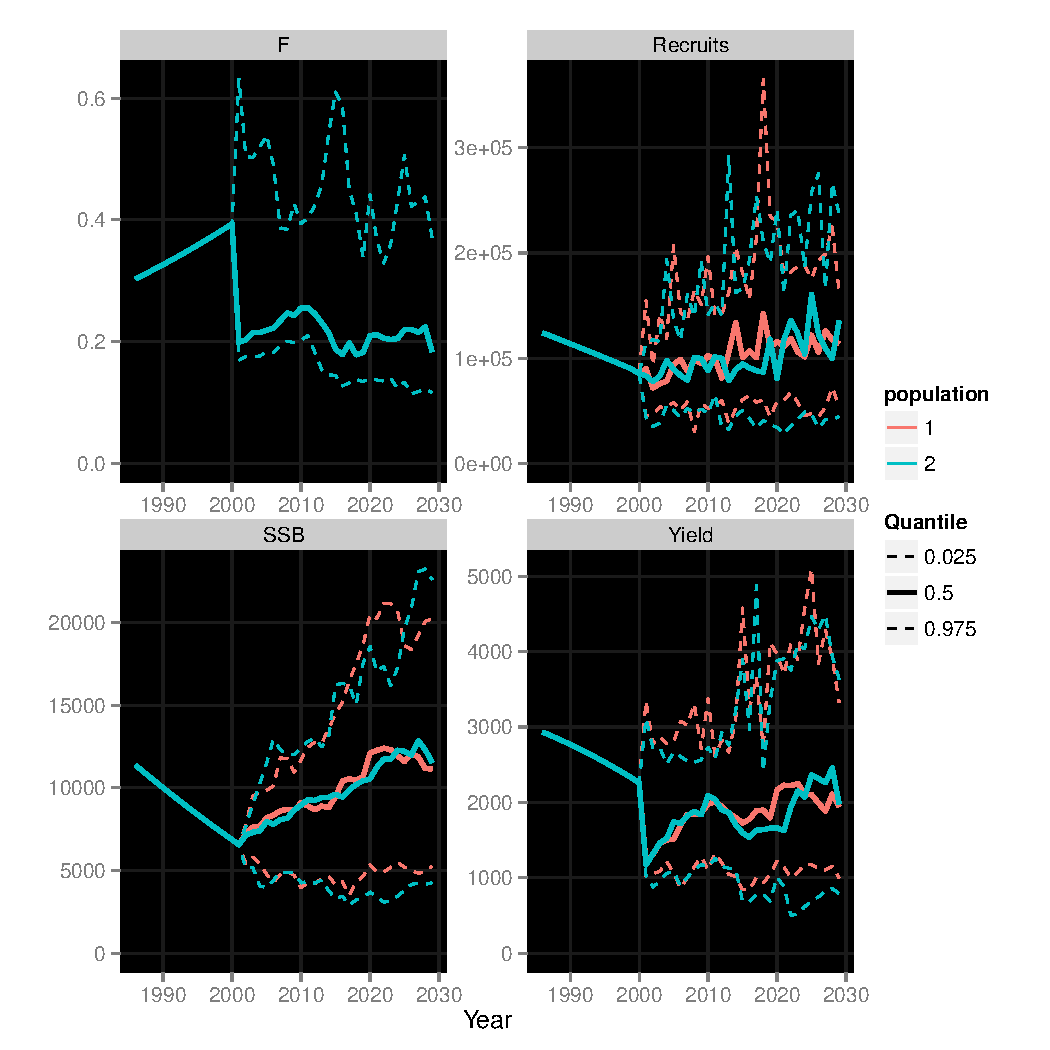
\includegraphics[width=.7\textwidth]{full-result1}
  \end{figure}
\end{frame}
\end{withoutheadline}

\begin{withoutheadline}
\begin{frame}{Results}
  Linf = 60 and Linf = 100 both with low Ricker recruitment
  \begin{figure}
  \flushleft
  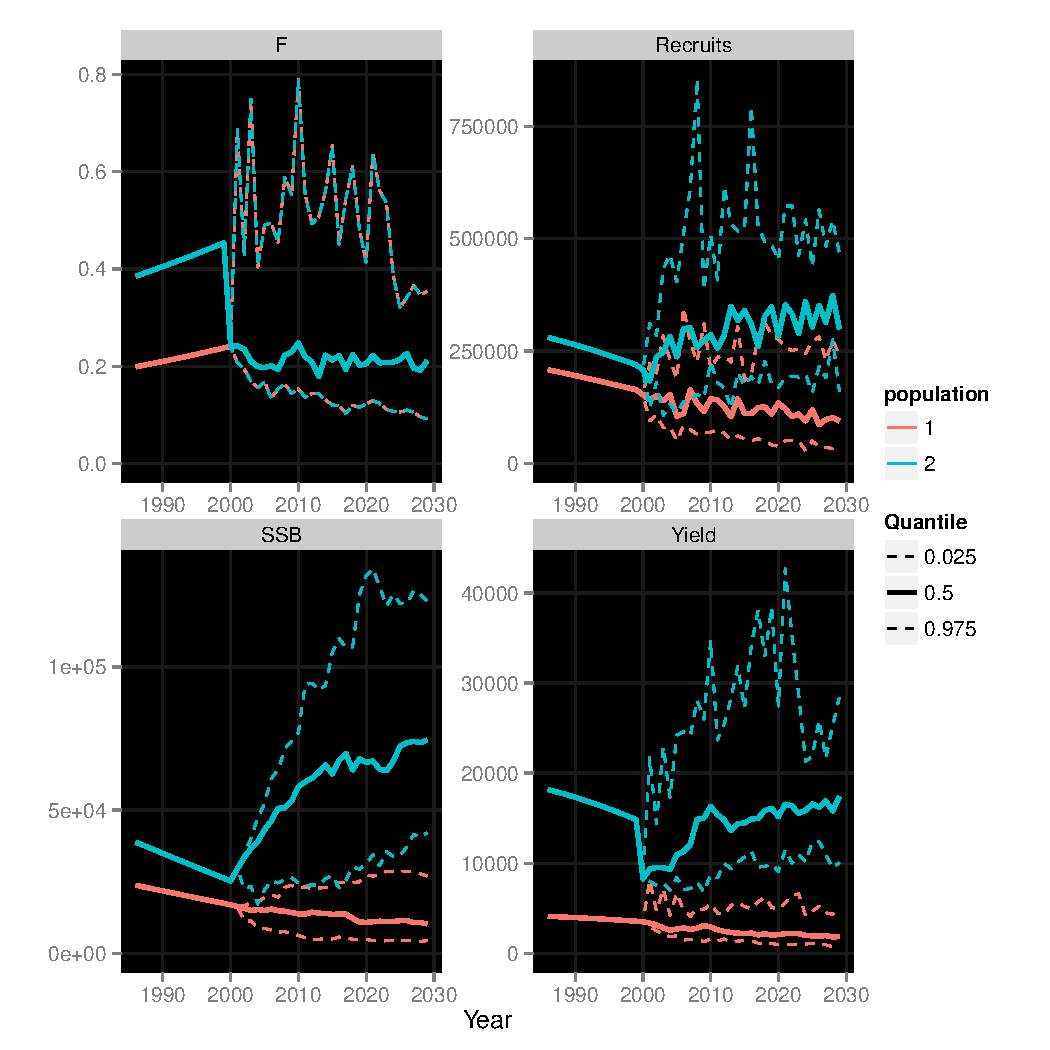
\includegraphics[width=.7\textwidth]{full-result2}
  \end{figure}
\end{frame}
\end{withoutheadline}

%%%%%%%%%%%%%%%%%%%%%%%%%%%%%%%%%%%%%%%%%%%%%


%\begin{withoutheadline}
%\begin{frame}{Results Summary: Stock Biomass Ratio}
%  \begin{minipage}{.25\textwidth}
%    2: L60 Low \\
%    3: L80 Low \\
%    4: L100 Low \\\\
%    5: L60 High \\
%    6: L80 High \\
%    7: L100 High \\\\
%    lower tri: Ricker \\
%    upper tri: BevHolt
%  \end{minipage}
%  \hspace{.25cm}
%  \begin{minipage}{0.7\textwidth}
%  \begin{figure}
%  \includegraphics[width=\textwidth]{tmat}
%  \end{figure}
%  \end{minipage}
%\end{frame}
%\end{withoutheadline}

\begin{withoutheadline}
\begin{frame}{Ecosystem Changes}
  Changes in total stock biomass ratio
  \begin{figure}
  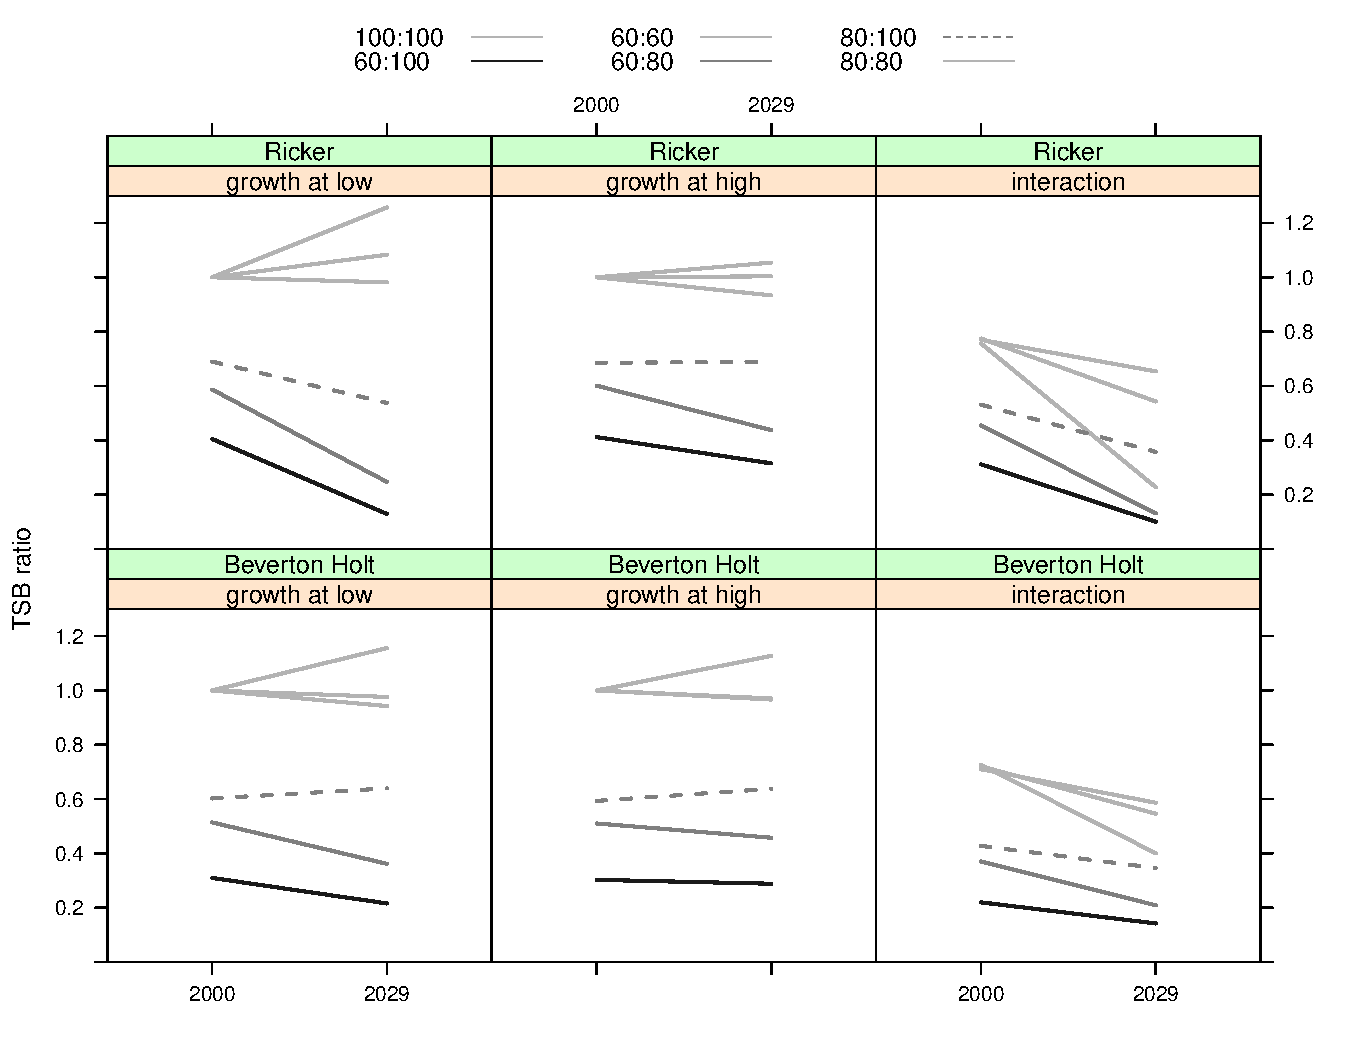
\includegraphics[width=.8\textwidth]{Bratio-plot}
  \end{figure}
\end{frame}
\end{withoutheadline}


\begin{withoutheadline}
\begin{frame}{Relative stock status in 2029}
    Stock status $S = B/B_{msy}$, relative stock status = $S_1/S_2$
  \begin{figure}
  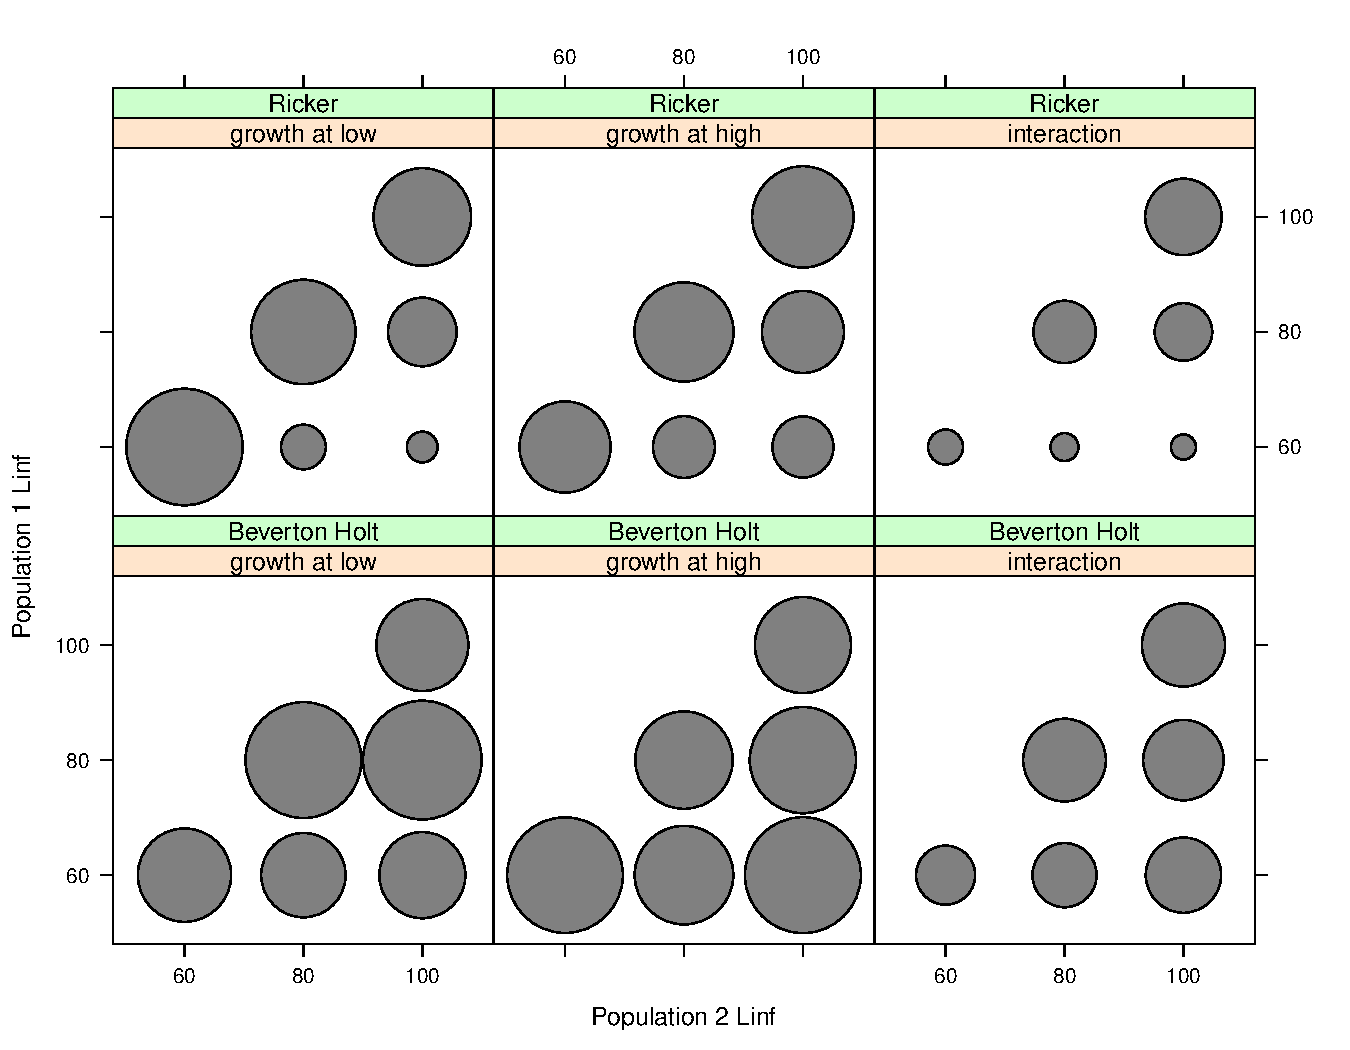
\includegraphics[width=.8\textwidth]{Bmsy-plot}
  \end{figure}
\end{frame}
\end{withoutheadline}


%\begin{withoutheadline}
%\begin{frame}{B/Bmsy ratio vs F/Fmsy ratio}
%  \begin{figure}
%  \includegraphics[width=.65\textwidth]{stock-plot}
%  \end{figure}
%\end{frame}
%\end{withoutheadline}


%%%%%%%%%%%%%%%%%%%%%%%%%%%%%%%%%%%%%%%%%%%%%

\begin{frame}{Final Thoughts}
  \begin{itemize}
    \item Not considering stock structure can result in serious \textbf{over exploitation}
    \item \textbf{Depensation effects} make for stronger impacts on sub unit mismanagement
    \item Develop automatic \textbf{HCRs} that can cope with stock structure
    \item Ongoing work:    
     \begin{itemize}
      \item Investigate other LH parameter sets
      \item Explore links between: virgin biomass and M, Recruitment with Fmsy and Fcrash etc. 
      \item Investigate alternative HCRs
     \end{itemize}         
  \end{itemize}
\end{frame}

%%%%%%%%%%%%%%%%%%%%%%%%%%%%%%%%%%%%%%%%%%%%%

\end{document}
